\documentclass[12pt]{article}
\usepackage[utf8]{inputenc}
\usepackage[spanish]{babel}
\usepackage{graphicx}
\usepackage{amsmath}
\usepackage{amssymb}
\usepackage{array}
\usepackage{xcolor}
\usepackage{geometry}
\usepackage{fancyhdr}
\usepackage{lastpage}
\usepackage{booktabs}
\usepackage{colortbl}
\usepackage{caption}
\usepackage{multirow}
\geometry{margin=1in}

\usepackage{float}
\definecolor{lightblue}{RGB}{200,230,255}
\definecolor{lightgreen}{RGB}{220,255,220}
\definecolor{lightred}{RGB}{255,220,220}
\definecolor{lightyellow}{RGB}{255,255,200}
\pagestyle{fancy}
\fancyhf{}
\fancyhead[L]{Algoritmo de Floyd - Solución}
\fancyhead[R]{\thepage\ de \pageref{LastPage}}
\renewcommand{\headrulewidth}{0.4pt}
\renewcommand{\footrulewidth}{0.4pt}

\title{Proyecto 1: Rutas Optimas (Algoritmo de Floyd)}
\author{Emily Sanchez \\ Viviana Vargas \\[1cm] Curso: Investigación de Operaciones \\ II Semestre 2025}
\date{\today}

\begin{document}

\maketitle
\thispagestyle{empty}
\newpage
\setcounter{page}{1}

\section{Introducción}
El algoritmo de Floyd-Warshall es un algoritmo para encontrar los caminos más cortos en un grafo ponderado. Fue publicado por Robert Floyd en 1962.\\
El algoritmo de Floyd se basa en el principio de la Programación Dinámica.\\
\textbf{Complejidad espacial:} $O(n^2)$\\
\textbf{Complejidad temporal:} $O(n^3)$\\
\clearpage
\section{Descripción del Problema}
Grafo con 11 nodos:

\begin{itemize}
\item Nodo A: A
\item Nodo B: B
\item Nodo C: C
\item Nodo D: D
\item Nodo E: E
\item Nodo F: F
\item Nodo G: G
\item Nodo H: GSDHC
\item Nodo I: COLI
\item Nodo J: COLJ
\item Nodo K: K
\end{itemize}

\begin{figure}[h!]
\centering
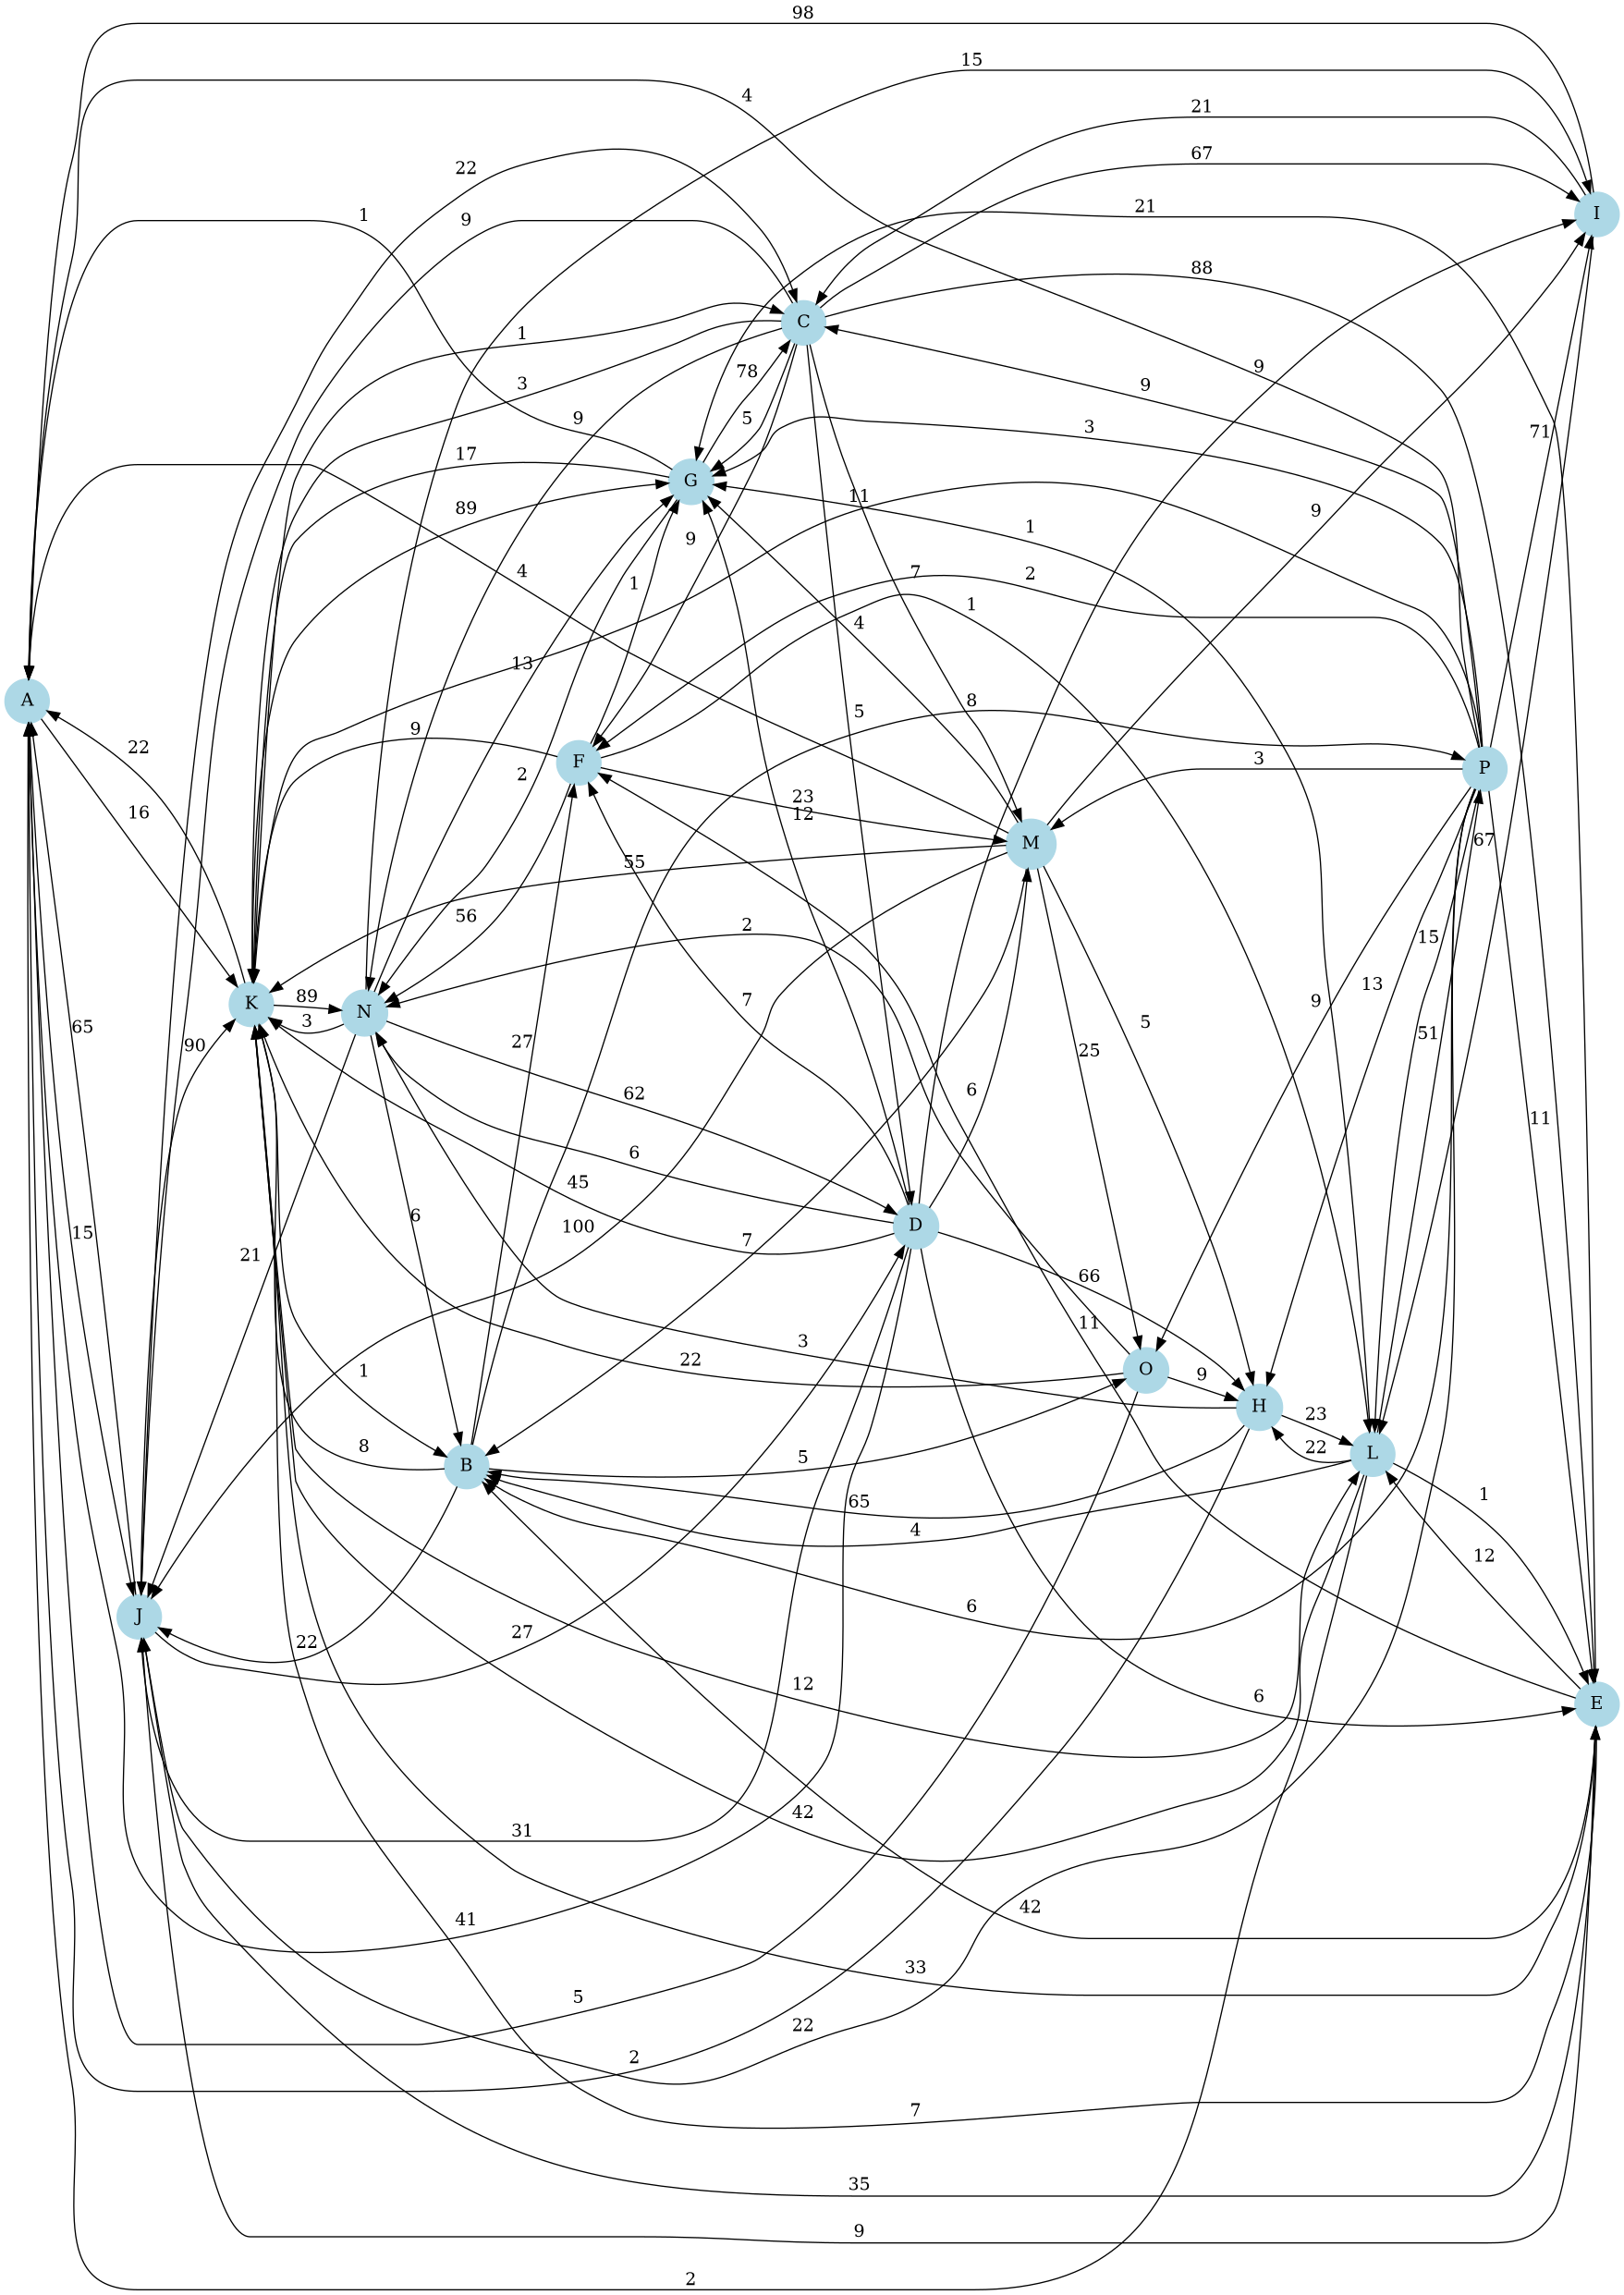
\includegraphics[width=0.5\textwidth,keepaspectratio]{grafo.png}
\caption{Representación del grafo original}
\end{figure}

\clearpage
\section{Procedimiento del Algoritmo}
\subsection{Matriz de Distancias Inicial D(0)}
\begin{table}[h!]
\centering
\begin{tabular}{|c|c|c|c|c|c|c|c|c|c|c|c|}
\hline
 & A & B & C & D & E & F & G & GSDHC & COLI & COLJ & K \\\hline
A & 0 & $\infty$ & 23 & $\infty$ & 1 & 1 & $\infty$ & $\infty$ & 1 & $\infty$ & 1 \\\hline
B & 12 & 0 & 2 & $\infty$ & $\infty$ & 1 & $\infty$ & $\infty$ & $\infty$ & $\infty$ & 12 \\\hline
C & $\infty$ & 1 & 0 & $\infty$ & 5 & $\infty$ & 6 & $\infty$ & 21 & 45 & 1 \\\hline
D & 67 & 1 & $\infty$ & 0 & 6 & 9 & $\infty$ & 21 & 12 & 1 & 2 \\\hline
E & 5 & $\infty$ & $\infty$ & $\infty$ & 0 & 11 & 5 & $\infty$ & 1 & 3 & 3 \\\hline
F & 5 & 2 & 10 & $\infty$ & $\infty$ & 0 & 2 & $\infty$ & $\infty$ & 45 & 2 \\\hline
G & 2 & $\infty$ & 9 & $\infty$ & $\infty$ & 11 & 0 & $\infty$ & 9 & 8 & $\infty$ \\\hline
GSDHC & 3 & 7 & 8 & $\infty$ & 16 & 21 & 30 & 0 & 23 & 7 & $\infty$ \\\hline
COLI & $\infty$ & $\infty$ & $\infty$ & $\infty$ & $\infty$ & $\infty$ & $\infty$ & $\infty$ & 0 & 6 & 15 \\\hline
COLJ & 90 & 21 & $\infty$ & $\infty$ & $\infty$ & $\infty$ & $\infty$ & 2 & 3 & 0 & $\infty$ \\\hline
K & 1 & 34 & $\infty$ & $\infty$ & $\infty$ & $\infty$ & $\infty$ & $\infty$ & 4 & 5 & 0 \\\hline
\end{tabular}
\caption{Matriz de distancias inicial D(0)}
\end{table}

\clearpage
\subsection{Matriz de Caminos Inicial P(0)}
\begin{table}[h!]
\centering
\begin{tabular}{|c|c|c|c|c|c|c|c|c|c|c|c|}
\hline
 & A & B & C & D & E & F & G & GSDHC & COLI & COLJ & K \\\hline
A & - & - & A & - & A & A & - & - & A & - & A \\\hline
B & B & - & B & - & - & B & - & - & - & - & B \\\hline
C & - & C & - & - & C & - & C & - & C & C & C \\\hline
D & D & D & - & - & D & D & - & D & D & D & D \\\hline
E & E & - & - & - & - & E & E & - & E & E & E \\\hline
F & F & F & F & - & - & - & F & - & - & F & F \\\hline
G & G & - & G & - & - & G & - & - & G & G & - \\\hline
GSDHC & GSDHC & GSDHC & GSDHC & - & GSDHC & GSDHC & GSDHC & - & GSDHC & GSDHC & - \\\hline
COLI & - & - & - & - & - & - & - & - & - & COLI & COLI \\\hline
COLJ & COLJ & COLJ & - & - & - & - & - & COLJ & COLJ & - & - \\\hline
K & K & K & - & - & - & - & - & - & K & K & - \\\hline
\end{tabular}
\caption{Matriz de caminos inicial P(0)}
\end{table}

\clearpage
\subsection{Iteraciones del Algoritmo}
\subsubsection{Iteración 1 (k = 1) - Nodo intermedio: A}
\paragraph{Matriz de Distancias D(1)}
\begin{table}[h!]
\centering
\begin{tabular}{|c|c|c|c|c|c|c|c|c|c|c|c|}
\hline
 & A & B & C & D & E & F & G & GSDHC & COLI & COLJ & K \\\hline
A & 0 & $\infty$ & 23 & $\infty$ & 1 & 1 & $\infty$ & $\infty$ & 1 & $\infty$ & 1 \\\hline
B & 12 & 0 & 2 & $\infty$ & \cellcolor{lightgreen} 13 & 1 & $\infty$ & $\infty$ & \cellcolor{lightgreen} 13 & $\infty$ & 12 \\\hline
C & $\infty$ & 1 & 0 & $\infty$ & 5 & $\infty$ & 6 & $\infty$ & 21 & 45 & 1 \\\hline
D & 67 & 1 & \cellcolor{lightgreen} 90 & 0 & 6 & 9 & $\infty$ & 21 & 12 & 1 & 2 \\\hline
E & 5 & $\infty$ & \cellcolor{lightgreen} 28 & $\infty$ & 0 & \cellcolor{lightgreen} 6 & 5 & $\infty$ & 1 & 3 & 3 \\\hline
F & 5 & 2 & 10 & $\infty$ & \cellcolor{lightgreen} 6 & 0 & 2 & $\infty$ & \cellcolor{lightgreen} 6 & 45 & 2 \\\hline
G & 2 & $\infty$ & 9 & $\infty$ & \cellcolor{lightgreen} 3 & \cellcolor{lightgreen} 3 & 0 & $\infty$ & \cellcolor{lightgreen} 3 & 8 & \cellcolor{lightgreen} 3 \\\hline
GSDHC & 3 & 7 & 8 & $\infty$ & \cellcolor{lightgreen} 4 & \cellcolor{lightgreen} 4 & 30 & 0 & \cellcolor{lightgreen} 4 & 7 & \cellcolor{lightgreen} 4 \\\hline
COLI & $\infty$ & $\infty$ & $\infty$ & $\infty$ & $\infty$ & $\infty$ & $\infty$ & $\infty$ & 0 & 6 & 15 \\\hline
COLJ & 90 & 21 & \cellcolor{lightgreen} 113 & $\infty$ & \cellcolor{lightgreen} 91 & \cellcolor{lightgreen} 91 & $\infty$ & 2 & 3 & 0 & \cellcolor{lightgreen} 91 \\\hline
K & 1 & 34 & \cellcolor{lightgreen} 24 & $\infty$ & \cellcolor{lightgreen} 2 & \cellcolor{lightgreen} 2 & $\infty$ & $\infty$ & \cellcolor{lightgreen} 2 & 5 & 0 \\\hline
\end{tabular}
\caption{Matriz de distancias D(1) - Cambios resaltados en verde}
\end{table}

\paragraph{Matriz de Caminos P(1)}
\begin{table}[h!]
\centering
\begin{tabular}{|c|c|c|c|c|c|c|c|c|c|c|c|}
\hline
 & A & B & C & D & E & F & G & GSDHC & COLI & COLJ & K \\\hline
A & - & - & A & - & A & A & - & - & A & - & A \\\hline
B & B & - & B & - & \cellcolor{lightblue} A & B & - & - & \cellcolor{lightblue} A & - & B \\\hline
C & - & C & - & - & C & - & C & - & C & C & C \\\hline
D & D & D & \cellcolor{lightblue} A & - & D & D & - & D & D & D & D \\\hline
E & E & - & \cellcolor{lightblue} A & - & - & \cellcolor{lightblue} A & E & - & E & E & E \\\hline
F & F & F & F & - & \cellcolor{lightblue} A & - & F & - & \cellcolor{lightblue} A & F & F \\\hline
G & G & - & G & - & \cellcolor{lightblue} A & \cellcolor{lightblue} A & - & - & \cellcolor{lightblue} A & G & \cellcolor{lightblue} A \\\hline
GSDHC & GSDHC & GSDHC & GSDHC & - & \cellcolor{lightblue} A & \cellcolor{lightblue} A & GSDHC & - & \cellcolor{lightblue} A & GSDHC & \cellcolor{lightblue} A \\\hline
COLI & - & - & - & - & - & - & - & - & - & COLI & COLI \\\hline
COLJ & COLJ & COLJ & \cellcolor{lightblue} A & - & \cellcolor{lightblue} A & \cellcolor{lightblue} A & - & COLJ & COLJ & - & \cellcolor{lightblue} A \\\hline
K & K & K & \cellcolor{lightblue} A & - & \cellcolor{lightblue} A & \cellcolor{lightblue} A & - & - & \cellcolor{lightblue} A & K & - \\\hline
\end{tabular}
\caption{Matriz de caminos P(1) - Cambios resaltados en azul}
\end{table}

\subsubsection{Iteración 2 (k = 2) - Nodo intermedio: B}
\paragraph{Matriz de Distancias D(2)}
\begin{table}[h!]
\centering
\begin{tabular}{|c|c|c|c|c|c|c|c|c|c|c|c|}
\hline
 & A & B & C & D & E & F & G & GSDHC & COLI & COLJ & K \\\hline
A & 0 & $\infty$ & 23 & $\infty$ & 1 & 1 & $\infty$ & $\infty$ & 1 & $\infty$ & 1 \\\hline
B & 12 & 0 & 2 & $\infty$ & 13 & 1 & $\infty$ & $\infty$ & 13 & $\infty$ & 12 \\\hline
C & \cellcolor{lightgreen} 13 & 1 & 0 & $\infty$ & 5 & \cellcolor{lightgreen} 2 & 6 & $\infty$ & \cellcolor{lightgreen} 14 & 45 & 1 \\\hline
D & \cellcolor{lightgreen} 13 & 1 & \cellcolor{lightgreen} 3 & 0 & 6 & \cellcolor{lightgreen} 2 & $\infty$ & 21 & 12 & 1 & 2 \\\hline
E & 5 & $\infty$ & 28 & $\infty$ & 0 & 6 & 5 & $\infty$ & 1 & 3 & 3 \\\hline
F & 5 & 2 & \cellcolor{lightgreen} 4 & $\infty$ & 6 & 0 & 2 & $\infty$ & 6 & 45 & 2 \\\hline
G & 2 & $\infty$ & 9 & $\infty$ & 3 & 3 & 0 & $\infty$ & 3 & 8 & 3 \\\hline
GSDHC & 3 & 7 & 8 & $\infty$ & 4 & 4 & 30 & 0 & 4 & 7 & 4 \\\hline
COLI & $\infty$ & $\infty$ & $\infty$ & $\infty$ & $\infty$ & $\infty$ & $\infty$ & $\infty$ & 0 & 6 & 15 \\\hline
COLJ & \cellcolor{lightgreen} 33 & 21 & \cellcolor{lightgreen} 23 & $\infty$ & \cellcolor{lightgreen} 34 & \cellcolor{lightgreen} 22 & $\infty$ & 2 & 3 & 0 & \cellcolor{lightgreen} 33 \\\hline
K & 1 & 34 & 24 & $\infty$ & 2 & 2 & $\infty$ & $\infty$ & 2 & 5 & 0 \\\hline
\end{tabular}
\caption{Matriz de distancias D(2) - Cambios resaltados en verde}
\end{table}

\paragraph{Matriz de Caminos P(2)}
\begin{table}[h!]
\centering
\begin{tabular}{|c|c|c|c|c|c|c|c|c|c|c|c|}
\hline
 & A & B & C & D & E & F & G & GSDHC & COLI & COLJ & K \\\hline
A & - & - & A & - & A & A & - & - & A & - & A \\\hline
B & B & - & B & - & A & B & - & - & A & - & B \\\hline
C & \cellcolor{lightblue} B & C & - & - & C & \cellcolor{lightblue} B & C & - & \cellcolor{lightblue} A & C & C \\\hline
D & \cellcolor{lightblue} B & D & \cellcolor{lightblue} B & - & D & \cellcolor{lightblue} B & - & D & D & D & D \\\hline
E & E & - & A & - & - & A & E & - & E & E & E \\\hline
F & F & F & \cellcolor{lightblue} B & - & A & - & F & - & A & F & F \\\hline
G & G & - & G & - & A & A & - & - & A & G & A \\\hline
GSDHC & GSDHC & GSDHC & GSDHC & - & A & A & GSDHC & - & A & GSDHC & A \\\hline
COLI & - & - & - & - & - & - & - & - & - & COLI & COLI \\\hline
COLJ & \cellcolor{lightblue} B & COLJ & \cellcolor{lightblue} B & - & A & \cellcolor{lightblue} B & - & COLJ & COLJ & - & \cellcolor{lightblue} B \\\hline
K & K & K & A & - & A & A & - & - & A & K & - \\\hline
\end{tabular}
\caption{Matriz de caminos P(2) - Cambios resaltados en azul}
\end{table}

\subsubsection{Iteración 3 (k = 3) - Nodo intermedio: C}
\paragraph{Matriz de Distancias D(3)}
\begin{table}[h!]
\centering
\begin{tabular}{|c|c|c|c|c|c|c|c|c|c|c|c|}
\hline
 & A & B & C & D & E & F & G & GSDHC & COLI & COLJ & K \\\hline
A & 0 & \cellcolor{lightgreen} 24 & 23 & $\infty$ & 1 & 1 & \cellcolor{lightgreen} 29 & $\infty$ & 1 & \cellcolor{lightgreen} 68 & 1 \\\hline
B & 12 & 0 & 2 & $\infty$ & \cellcolor{lightgreen} 7 & 1 & \cellcolor{lightgreen} 8 & $\infty$ & 13 & \cellcolor{lightgreen} 47 & \cellcolor{lightgreen} 3 \\\hline
C & 13 & 1 & 0 & $\infty$ & 5 & 2 & 6 & $\infty$ & 14 & 45 & 1 \\\hline
D & 13 & 1 & 3 & 0 & 6 & 2 & \cellcolor{lightgreen} 9 & 21 & 12 & 1 & 2 \\\hline
E & 5 & \cellcolor{lightgreen} 29 & 28 & $\infty$ & 0 & 6 & 5 & $\infty$ & 1 & 3 & 3 \\\hline
F & 5 & 2 & 4 & $\infty$ & 6 & 0 & 2 & $\infty$ & 6 & 45 & 2 \\\hline
G & 2 & \cellcolor{lightgreen} 10 & 9 & $\infty$ & 3 & 3 & 0 & $\infty$ & 3 & 8 & 3 \\\hline
GSDHC & 3 & 7 & 8 & $\infty$ & 4 & 4 & \cellcolor{lightgreen} 14 & 0 & 4 & 7 & 4 \\\hline
COLI & $\infty$ & $\infty$ & $\infty$ & $\infty$ & $\infty$ & $\infty$ & $\infty$ & $\infty$ & 0 & 6 & 15 \\\hline
COLJ & 33 & 21 & 23 & $\infty$ & \cellcolor{lightgreen} 28 & 22 & \cellcolor{lightgreen} 29 & 2 & 3 & 0 & \cellcolor{lightgreen} 24 \\\hline
K & 1 & \cellcolor{lightgreen} 25 & 24 & $\infty$ & 2 & 2 & \cellcolor{lightgreen} 30 & $\infty$ & 2 & 5 & 0 \\\hline
\end{tabular}
\caption{Matriz de distancias D(3) - Cambios resaltados en verde}
\end{table}

\paragraph{Matriz de Caminos P(3)}
\begin{table}[h!]
\centering
\begin{tabular}{|c|c|c|c|c|c|c|c|c|c|c|c|}
\hline
 & A & B & C & D & E & F & G & GSDHC & COLI & COLJ & K \\\hline
A & - & \cellcolor{lightblue} C & A & - & A & A & \cellcolor{lightblue} C & - & A & \cellcolor{lightblue} C & A \\\hline
B & B & - & B & - & \cellcolor{lightblue} C & B & \cellcolor{lightblue} C & - & A & \cellcolor{lightblue} C & \cellcolor{lightblue} C \\\hline
C & B & C & - & - & C & B & C & - & A & C & C \\\hline
D & B & D & B & - & D & B & \cellcolor{lightblue} C & D & D & D & D \\\hline
E & E & \cellcolor{lightblue} C & A & - & - & A & E & - & E & E & E \\\hline
F & F & F & B & - & A & - & F & - & A & F & F \\\hline
G & G & \cellcolor{lightblue} C & G & - & A & A & - & - & A & G & A \\\hline
GSDHC & GSDHC & GSDHC & GSDHC & - & A & A & \cellcolor{lightblue} C & - & A & GSDHC & A \\\hline
COLI & - & - & - & - & - & - & - & - & - & COLI & COLI \\\hline
COLJ & B & COLJ & B & - & \cellcolor{lightblue} C & B & \cellcolor{lightblue} C & COLJ & COLJ & - & \cellcolor{lightblue} C \\\hline
K & K & \cellcolor{lightblue} C & A & - & A & A & \cellcolor{lightblue} C & - & A & K & - \\\hline
\end{tabular}
\caption{Matriz de caminos P(3) - Cambios resaltados en azul}
\end{table}

\subsubsection{Iteración 4 (k = 4) - Nodo intermedio: D}
\paragraph{Matriz de Distancias D(4)}
\begin{table}[h!]
\centering
\begin{tabular}{|c|c|c|c|c|c|c|c|c|c|c|c|}
\hline
 & A & B & C & D & E & F & G & GSDHC & COLI & COLJ & K \\\hline
A & 0 & 24 & 23 & $\infty$ & 1 & 1 & 29 & $\infty$ & 1 & 68 & 1 \\\hline
B & 12 & 0 & 2 & $\infty$ & 7 & 1 & 8 & $\infty$ & 13 & 47 & 3 \\\hline
C & 13 & 1 & 0 & $\infty$ & 5 & 2 & 6 & $\infty$ & 14 & 45 & 1 \\\hline
D & 13 & 1 & 3 & 0 & 6 & 2 & 9 & 21 & 12 & 1 & 2 \\\hline
E & 5 & 29 & 28 & $\infty$ & 0 & 6 & 5 & $\infty$ & 1 & 3 & 3 \\\hline
F & 5 & 2 & 4 & $\infty$ & 6 & 0 & 2 & $\infty$ & 6 & 45 & 2 \\\hline
G & 2 & 10 & 9 & $\infty$ & 3 & 3 & 0 & $\infty$ & 3 & 8 & 3 \\\hline
GSDHC & 3 & 7 & 8 & $\infty$ & 4 & 4 & 14 & 0 & 4 & 7 & 4 \\\hline
COLI & $\infty$ & $\infty$ & $\infty$ & $\infty$ & $\infty$ & $\infty$ & $\infty$ & $\infty$ & 0 & 6 & 15 \\\hline
COLJ & 33 & 21 & 23 & $\infty$ & 28 & 22 & 29 & 2 & 3 & 0 & 24 \\\hline
K & 1 & 25 & 24 & $\infty$ & 2 & 2 & 30 & $\infty$ & 2 & 5 & 0 \\\hline
\end{tabular}
\caption{Matriz de distancias D(4) - Cambios resaltados en verde}
\end{table}

\paragraph{Matriz de Caminos P(4)}
\begin{table}[h!]
\centering
\begin{tabular}{|c|c|c|c|c|c|c|c|c|c|c|c|}
\hline
 & A & B & C & D & E & F & G & GSDHC & COLI & COLJ & K \\\hline
A & - & C & A & - & A & A & C & - & A & C & A \\\hline
B & B & - & B & - & C & B & C & - & A & C & C \\\hline
C & B & C & - & - & C & B & C & - & A & C & C \\\hline
D & B & D & B & - & D & B & C & D & D & D & D \\\hline
E & E & C & A & - & - & A & E & - & E & E & E \\\hline
F & F & F & B & - & A & - & F & - & A & F & F \\\hline
G & G & C & G & - & A & A & - & - & A & G & A \\\hline
GSDHC & GSDHC & GSDHC & GSDHC & - & A & A & C & - & A & GSDHC & A \\\hline
COLI & - & - & - & - & - & - & - & - & - & COLI & COLI \\\hline
COLJ & B & COLJ & B & - & C & B & C & COLJ & COLJ & - & C \\\hline
K & K & C & A & - & A & A & C & - & A & K & - \\\hline
\end{tabular}
\caption{Matriz de caminos P(4) - Cambios resaltados en azul}
\end{table}

\subsubsection{Iteración 5 (k = 5) - Nodo intermedio: E}
\paragraph{Matriz de Distancias D(5)}
\begin{table}[h!]
\centering
\begin{tabular}{|c|c|c|c|c|c|c|c|c|c|c|c|}
\hline
 & A & B & C & D & E & F & G & GSDHC & COLI & COLJ & K \\\hline
A & 0 & 24 & 23 & $\infty$ & 1 & 1 & \cellcolor{lightgreen} 6 & $\infty$ & 1 & \cellcolor{lightgreen} 4 & 1 \\\hline
B & 12 & 0 & 2 & $\infty$ & 7 & 1 & 8 & $\infty$ & \cellcolor{lightgreen} 8 & \cellcolor{lightgreen} 10 & 3 \\\hline
C & \cellcolor{lightgreen} 10 & 1 & 0 & $\infty$ & 5 & 2 & 6 & $\infty$ & \cellcolor{lightgreen} 6 & \cellcolor{lightgreen} 8 & 1 \\\hline
D & \cellcolor{lightgreen} 11 & 1 & 3 & 0 & 6 & 2 & 9 & 21 & \cellcolor{lightgreen} 7 & 1 & 2 \\\hline
E & 5 & 29 & 28 & $\infty$ & 0 & 6 & 5 & $\infty$ & 1 & 3 & 3 \\\hline
F & 5 & 2 & 4 & $\infty$ & 6 & 0 & 2 & $\infty$ & 6 & \cellcolor{lightgreen} 9 & 2 \\\hline
G & 2 & 10 & 9 & $\infty$ & 3 & 3 & 0 & $\infty$ & 3 & \cellcolor{lightgreen} 6 & 3 \\\hline
GSDHC & 3 & 7 & 8 & $\infty$ & 4 & 4 & \cellcolor{lightgreen} 9 & 0 & 4 & 7 & 4 \\\hline
COLI & $\infty$ & $\infty$ & $\infty$ & $\infty$ & $\infty$ & $\infty$ & $\infty$ & $\infty$ & 0 & 6 & 15 \\\hline
COLJ & 33 & 21 & 23 & $\infty$ & 28 & 22 & 29 & 2 & 3 & 0 & 24 \\\hline
K & 1 & 25 & 24 & $\infty$ & 2 & 2 & \cellcolor{lightgreen} 7 & $\infty$ & 2 & 5 & 0 \\\hline
\end{tabular}
\caption{Matriz de distancias D(5) - Cambios resaltados en verde}
\end{table}

\paragraph{Matriz de Caminos P(5)}
\begin{table}[h!]
\centering
\begin{tabular}{|c|c|c|c|c|c|c|c|c|c|c|c|}
\hline
 & A & B & C & D & E & F & G & GSDHC & COLI & COLJ & K \\\hline
A & - & C & A & - & A & A & \cellcolor{lightblue} E & - & A & \cellcolor{lightblue} E & A \\\hline
B & B & - & B & - & C & B & C & - & \cellcolor{lightblue} E & \cellcolor{lightblue} E & C \\\hline
C & \cellcolor{lightblue} E & C & - & - & C & B & C & - & \cellcolor{lightblue} E & \cellcolor{lightblue} E & C \\\hline
D & \cellcolor{lightblue} E & D & B & - & D & B & C & D & \cellcolor{lightblue} E & D & D \\\hline
E & E & C & A & - & - & A & E & - & E & E & E \\\hline
F & F & F & B & - & A & - & F & - & A & \cellcolor{lightblue} E & F \\\hline
G & G & C & G & - & A & A & - & - & A & \cellcolor{lightblue} E & A \\\hline
GSDHC & GSDHC & GSDHC & GSDHC & - & A & A & \cellcolor{lightblue} E & - & A & GSDHC & A \\\hline
COLI & - & - & - & - & - & - & - & - & - & COLI & COLI \\\hline
COLJ & B & COLJ & B & - & C & B & C & COLJ & COLJ & - & C \\\hline
K & K & C & A & - & A & A & \cellcolor{lightblue} E & - & A & K & - \\\hline
\end{tabular}
\caption{Matriz de caminos P(5) - Cambios resaltados en azul}
\end{table}

\subsubsection{Iteración 6 (k = 6) - Nodo intermedio: F}
\paragraph{Matriz de Distancias D(6)}
\begin{table}[h!]
\centering
\begin{tabular}{|c|c|c|c|c|c|c|c|c|c|c|c|}
\hline
 & A & B & C & D & E & F & G & GSDHC & COLI & COLJ & K \\\hline
A & 0 & \cellcolor{lightgreen} 3 & \cellcolor{lightgreen} 5 & $\infty$ & 1 & 1 & \cellcolor{lightgreen} 3 & $\infty$ & 1 & 4 & 1 \\\hline
B & \cellcolor{lightgreen} 6 & 0 & 2 & $\infty$ & 7 & 1 & \cellcolor{lightgreen} 3 & $\infty$ & \cellcolor{lightgreen} 7 & 10 & 3 \\\hline
C & \cellcolor{lightgreen} 7 & 1 & 0 & $\infty$ & 5 & 2 & \cellcolor{lightgreen} 4 & $\infty$ & 6 & 8 & 1 \\\hline
D & \cellcolor{lightgreen} 7 & 1 & 3 & 0 & 6 & 2 & \cellcolor{lightgreen} 4 & 21 & 7 & 1 & 2 \\\hline
E & 5 & \cellcolor{lightgreen} 8 & \cellcolor{lightgreen} 10 & $\infty$ & 0 & 6 & 5 & $\infty$ & 1 & 3 & 3 \\\hline
F & 5 & 2 & 4 & $\infty$ & 6 & 0 & 2 & $\infty$ & 6 & 9 & 2 \\\hline
G & 2 & \cellcolor{lightgreen} 5 & \cellcolor{lightgreen} 7 & $\infty$ & 3 & 3 & 0 & $\infty$ & 3 & 6 & 3 \\\hline
GSDHC & 3 & \cellcolor{lightgreen} 6 & 8 & $\infty$ & 4 & 4 & \cellcolor{lightgreen} 6 & 0 & 4 & 7 & 4 \\\hline
COLI & $\infty$ & $\infty$ & $\infty$ & $\infty$ & $\infty$ & $\infty$ & $\infty$ & $\infty$ & 0 & 6 & 15 \\\hline
COLJ & \cellcolor{lightgreen} 27 & 21 & 23 & $\infty$ & 28 & 22 & \cellcolor{lightgreen} 24 & 2 & 3 & 0 & 24 \\\hline
K & 1 & \cellcolor{lightgreen} 4 & \cellcolor{lightgreen} 6 & $\infty$ & 2 & 2 & \cellcolor{lightgreen} 4 & $\infty$ & 2 & 5 & 0 \\\hline
\end{tabular}
\caption{Matriz de distancias D(6) - Cambios resaltados en verde}
\end{table}

\paragraph{Matriz de Caminos P(6)}
\begin{table}[h!]
\centering
\begin{tabular}{|c|c|c|c|c|c|c|c|c|c|c|c|}
\hline
 & A & B & C & D & E & F & G & GSDHC & COLI & COLJ & K \\\hline
A & - & \cellcolor{lightblue} F & \cellcolor{lightblue} B & - & A & A & \cellcolor{lightblue} F & - & A & E & A \\\hline
B & \cellcolor{lightblue} F & - & B & - & C & B & \cellcolor{lightblue} F & - & \cellcolor{lightblue} A & E & C \\\hline
C & \cellcolor{lightblue} F & C & - & - & C & B & \cellcolor{lightblue} F & - & E & E & C \\\hline
D & \cellcolor{lightblue} F & D & B & - & D & B & \cellcolor{lightblue} F & D & E & D & D \\\hline
E & E & \cellcolor{lightblue} F & \cellcolor{lightblue} B & - & - & A & E & - & E & E & E \\\hline
F & F & F & B & - & A & - & F & - & A & E & F \\\hline
G & G & \cellcolor{lightblue} F & \cellcolor{lightblue} B & - & A & A & - & - & A & E & A \\\hline
GSDHC & GSDHC & \cellcolor{lightblue} F & GSDHC & - & A & A & \cellcolor{lightblue} F & - & A & GSDHC & A \\\hline
COLI & - & - & - & - & - & - & - & - & - & COLI & COLI \\\hline
COLJ & \cellcolor{lightblue} F & COLJ & B & - & C & B & \cellcolor{lightblue} F & COLJ & COLJ & - & C \\\hline
K & K & \cellcolor{lightblue} F & \cellcolor{lightblue} B & - & A & A & \cellcolor{lightblue} F & - & A & K & - \\\hline
\end{tabular}
\caption{Matriz de caminos P(6) - Cambios resaltados en azul}
\end{table}

\subsubsection{Iteración 7 (k = 7) - Nodo intermedio: G}
\paragraph{Matriz de Distancias D(7)}
\begin{table}[h!]
\centering
\begin{tabular}{|c|c|c|c|c|c|c|c|c|c|c|c|}
\hline
 & A & B & C & D & E & F & G & GSDHC & COLI & COLJ & K \\\hline
A & 0 & 3 & 5 & $\infty$ & 1 & 1 & 3 & $\infty$ & 1 & 4 & 1 \\\hline
B & \cellcolor{lightgreen} 5 & 0 & 2 & $\infty$ & \cellcolor{lightgreen} 6 & 1 & 3 & $\infty$ & \cellcolor{lightgreen} 6 & \cellcolor{lightgreen} 9 & 3 \\\hline
C & \cellcolor{lightgreen} 6 & 1 & 0 & $\infty$ & 5 & 2 & 4 & $\infty$ & 6 & 8 & 1 \\\hline
D & \cellcolor{lightgreen} 6 & 1 & 3 & 0 & 6 & 2 & 4 & 21 & 7 & 1 & 2 \\\hline
E & 5 & 8 & 10 & $\infty$ & 0 & 6 & 5 & $\infty$ & 1 & 3 & 3 \\\hline
F & \cellcolor{lightgreen} 4 & 2 & 4 & $\infty$ & \cellcolor{lightgreen} 5 & 0 & 2 & $\infty$ & \cellcolor{lightgreen} 5 & \cellcolor{lightgreen} 8 & 2 \\\hline
G & 2 & 5 & 7 & $\infty$ & 3 & 3 & 0 & $\infty$ & 3 & 6 & 3 \\\hline
GSDHC & 3 & 6 & 8 & $\infty$ & 4 & 4 & 6 & 0 & 4 & 7 & 4 \\\hline
COLI & $\infty$ & $\infty$ & $\infty$ & $\infty$ & $\infty$ & $\infty$ & $\infty$ & $\infty$ & 0 & 6 & 15 \\\hline
COLJ & \cellcolor{lightgreen} 26 & 21 & 23 & $\infty$ & \cellcolor{lightgreen} 27 & 22 & 24 & 2 & 3 & 0 & 24 \\\hline
K & 1 & 4 & 6 & $\infty$ & 2 & 2 & 4 & $\infty$ & 2 & 5 & 0 \\\hline
\end{tabular}
\caption{Matriz de distancias D(7) - Cambios resaltados en verde}
\end{table}

\paragraph{Matriz de Caminos P(7)}
\begin{table}[h!]
\centering
\begin{tabular}{|c|c|c|c|c|c|c|c|c|c|c|c|}
\hline
 & A & B & C & D & E & F & G & GSDHC & COLI & COLJ & K \\\hline
A & - & F & B & - & A & A & F & - & A & E & A \\\hline
B & \cellcolor{lightblue} G & - & B & - & \cellcolor{lightblue} A & B & F & - & A & E & C \\\hline
C & \cellcolor{lightblue} G & C & - & - & C & B & F & - & E & E & C \\\hline
D & \cellcolor{lightblue} G & D & B & - & D & B & F & D & E & D & D \\\hline
E & E & F & B & - & - & A & E & - & E & E & E \\\hline
F & \cellcolor{lightblue} G & F & B & - & A & - & F & - & A & E & F \\\hline
G & G & F & B & - & A & A & - & - & A & E & A \\\hline
GSDHC & GSDHC & F & GSDHC & - & A & A & F & - & A & GSDHC & A \\\hline
COLI & - & - & - & - & - & - & - & - & - & COLI & COLI \\\hline
COLJ & \cellcolor{lightblue} G & COLJ & B & - & \cellcolor{lightblue} A & B & F & COLJ & COLJ & - & C \\\hline
K & K & F & B & - & A & A & F & - & A & K & - \\\hline
\end{tabular}
\caption{Matriz de caminos P(7) - Cambios resaltados en azul}
\end{table}

\subsubsection{Iteración 8 (k = 8) - Nodo intermedio: GSDHC}
\paragraph{Matriz de Distancias D(8)}
\begin{table}[h!]
\centering
\begin{tabular}{|c|c|c|c|c|c|c|c|c|c|c|c|}
\hline
 & A & B & C & D & E & F & G & GSDHC & COLI & COLJ & K \\\hline
A & 0 & 3 & 5 & $\infty$ & 1 & 1 & 3 & $\infty$ & 1 & 4 & 1 \\\hline
B & 5 & 0 & 2 & $\infty$ & 6 & 1 & 3 & $\infty$ & 6 & 9 & 3 \\\hline
C & 6 & 1 & 0 & $\infty$ & 5 & 2 & 4 & $\infty$ & 6 & 8 & 1 \\\hline
D & 6 & 1 & 3 & 0 & 6 & 2 & 4 & 21 & 7 & 1 & 2 \\\hline
E & 5 & 8 & 10 & $\infty$ & 0 & 6 & 5 & $\infty$ & 1 & 3 & 3 \\\hline
F & 4 & 2 & 4 & $\infty$ & 5 & 0 & 2 & $\infty$ & 5 & 8 & 2 \\\hline
G & 2 & 5 & 7 & $\infty$ & 3 & 3 & 0 & $\infty$ & 3 & 6 & 3 \\\hline
GSDHC & 3 & 6 & 8 & $\infty$ & 4 & 4 & 6 & 0 & 4 & 7 & 4 \\\hline
COLI & $\infty$ & $\infty$ & $\infty$ & $\infty$ & $\infty$ & $\infty$ & $\infty$ & $\infty$ & 0 & 6 & 15 \\\hline
COLJ & \cellcolor{lightgreen} 5 & \cellcolor{lightgreen} 8 & \cellcolor{lightgreen} 10 & $\infty$ & \cellcolor{lightgreen} 6 & \cellcolor{lightgreen} 6 & \cellcolor{lightgreen} 8 & 2 & 3 & 0 & \cellcolor{lightgreen} 6 \\\hline
K & 1 & 4 & 6 & $\infty$ & 2 & 2 & 4 & $\infty$ & 2 & 5 & 0 \\\hline
\end{tabular}
\caption{Matriz de distancias D(8) - Cambios resaltados en verde}
\end{table}

\paragraph{Matriz de Caminos P(8)}
\begin{table}[h!]
\centering
\begin{tabular}{|c|c|c|c|c|c|c|c|c|c|c|c|}
\hline
 & A & B & C & D & E & F & G & GSDHC & COLI & COLJ & K \\\hline
A & - & F & B & - & A & A & F & - & A & E & A \\\hline
B & G & - & B & - & A & B & F & - & A & E & C \\\hline
C & G & C & - & - & C & B & F & - & E & E & C \\\hline
D & G & D & B & - & D & B & F & D & E & D & D \\\hline
E & E & F & B & - & - & A & E & - & E & E & E \\\hline
F & G & F & B & - & A & - & F & - & A & E & F \\\hline
G & G & F & B & - & A & A & - & - & A & E & A \\\hline
GSDHC & GSDHC & F & GSDHC & - & A & A & F & - & A & GSDHC & A \\\hline
COLI & - & - & - & - & - & - & - & - & - & COLI & COLI \\\hline
COLJ & \cellcolor{lightblue} GSDHC & \cellcolor{lightblue} F & \cellcolor{lightblue} GSDHC & - & A & \cellcolor{lightblue} A & F & COLJ & COLJ & - & \cellcolor{lightblue} A \\\hline
K & K & F & B & - & A & A & F & - & A & K & - \\\hline
\end{tabular}
\caption{Matriz de caminos P(8) - Cambios resaltados en azul}
\end{table}

\subsubsection{Iteración 9 (k = 9) - Nodo intermedio: COLI}
\paragraph{Matriz de Distancias D(9)}
\begin{table}[h!]
\centering
\begin{tabular}{|c|c|c|c|c|c|c|c|c|c|c|c|}
\hline
 & A & B & C & D & E & F & G & GSDHC & COLI & COLJ & K \\\hline
A & 0 & 3 & 5 & $\infty$ & 1 & 1 & 3 & $\infty$ & 1 & 4 & 1 \\\hline
B & 5 & 0 & 2 & $\infty$ & 6 & 1 & 3 & $\infty$ & 6 & 9 & 3 \\\hline
C & 6 & 1 & 0 & $\infty$ & 5 & 2 & 4 & $\infty$ & 6 & 8 & 1 \\\hline
D & 6 & 1 & 3 & 0 & 6 & 2 & 4 & 21 & 7 & 1 & 2 \\\hline
E & 5 & 8 & 10 & $\infty$ & 0 & 6 & 5 & $\infty$ & 1 & 3 & 3 \\\hline
F & 4 & 2 & 4 & $\infty$ & 5 & 0 & 2 & $\infty$ & 5 & 8 & 2 \\\hline
G & 2 & 5 & 7 & $\infty$ & 3 & 3 & 0 & $\infty$ & 3 & 6 & 3 \\\hline
GSDHC & 3 & 6 & 8 & $\infty$ & 4 & 4 & 6 & 0 & 4 & 7 & 4 \\\hline
COLI & $\infty$ & $\infty$ & $\infty$ & $\infty$ & $\infty$ & $\infty$ & $\infty$ & $\infty$ & 0 & 6 & 15 \\\hline
COLJ & 5 & 8 & 10 & $\infty$ & 6 & 6 & 8 & 2 & 3 & 0 & 6 \\\hline
K & 1 & 4 & 6 & $\infty$ & 2 & 2 & 4 & $\infty$ & 2 & 5 & 0 \\\hline
\end{tabular}
\caption{Matriz de distancias D(9) - Cambios resaltados en verde}
\end{table}

\paragraph{Matriz de Caminos P(9)}
\begin{table}[h!]
\centering
\begin{tabular}{|c|c|c|c|c|c|c|c|c|c|c|c|}
\hline
 & A & B & C & D & E & F & G & GSDHC & COLI & COLJ & K \\\hline
A & - & F & B & - & A & A & F & - & A & E & A \\\hline
B & G & - & B & - & A & B & F & - & A & E & C \\\hline
C & G & C & - & - & C & B & F & - & E & E & C \\\hline
D & G & D & B & - & D & B & F & D & E & D & D \\\hline
E & E & F & B & - & - & A & E & - & E & E & E \\\hline
F & G & F & B & - & A & - & F & - & A & E & F \\\hline
G & G & F & B & - & A & A & - & - & A & E & A \\\hline
GSDHC & GSDHC & F & GSDHC & - & A & A & F & - & A & GSDHC & A \\\hline
COLI & - & - & - & - & - & - & - & - & - & COLI & COLI \\\hline
COLJ & GSDHC & F & GSDHC & - & A & A & F & COLJ & COLJ & - & A \\\hline
K & K & F & B & - & A & A & F & - & A & K & - \\\hline
\end{tabular}
\caption{Matriz de caminos P(9) - Cambios resaltados en azul}
\end{table}

\subsubsection{Iteración 10 (k = 10) - Nodo intermedio: COLJ}
\paragraph{Matriz de Distancias D(10)}
\begin{table}[h!]
\centering
\begin{tabular}{|c|c|c|c|c|c|c|c|c|c|c|c|}
\hline
 & A & B & C & D & E & F & G & GSDHC & COLI & COLJ & K \\\hline
A & 0 & 3 & 5 & $\infty$ & 1 & 1 & 3 & \cellcolor{lightgreen} 6 & 1 & 4 & 1 \\\hline
B & 5 & 0 & 2 & $\infty$ & 6 & 1 & 3 & \cellcolor{lightgreen} 11 & 6 & 9 & 3 \\\hline
C & 6 & 1 & 0 & $\infty$ & 5 & 2 & 4 & \cellcolor{lightgreen} 10 & 6 & 8 & 1 \\\hline
D & 6 & 1 & 3 & 0 & 6 & 2 & 4 & \cellcolor{lightgreen} 3 & \cellcolor{lightgreen} 4 & 1 & 2 \\\hline
E & 5 & 8 & 10 & $\infty$ & 0 & 6 & 5 & \cellcolor{lightgreen} 5 & 1 & 3 & 3 \\\hline
F & 4 & 2 & 4 & $\infty$ & 5 & 0 & 2 & \cellcolor{lightgreen} 10 & 5 & 8 & 2 \\\hline
G & 2 & 5 & 7 & $\infty$ & 3 & 3 & 0 & \cellcolor{lightgreen} 8 & 3 & 6 & 3 \\\hline
GSDHC & 3 & 6 & 8 & $\infty$ & 4 & 4 & 6 & 0 & 4 & 7 & 4 \\\hline
COLI & \cellcolor{lightgreen} 11 & \cellcolor{lightgreen} 14 & \cellcolor{lightgreen} 16 & $\infty$ & \cellcolor{lightgreen} 12 & \cellcolor{lightgreen} 12 & \cellcolor{lightgreen} 14 & \cellcolor{lightgreen} 8 & 0 & 6 & \cellcolor{lightgreen} 12 \\\hline
COLJ & 5 & 8 & 10 & $\infty$ & 6 & 6 & 8 & 2 & 3 & 0 & 6 \\\hline
K & 1 & 4 & 6 & $\infty$ & 2 & 2 & 4 & \cellcolor{lightgreen} 7 & 2 & 5 & 0 \\\hline
\end{tabular}
\caption{Matriz de distancias D(10) - Cambios resaltados en verde}
\end{table}

\paragraph{Matriz de Caminos P(10)}
\begin{table}[h!]
\centering
\begin{tabular}{|c|c|c|c|c|c|c|c|c|c|c|c|}
\hline
 & A & B & C & D & E & F & G & GSDHC & COLI & COLJ & K \\\hline
A & - & F & B & - & A & A & F & \cellcolor{lightblue} COLJ & A & E & A \\\hline
B & G & - & B & - & A & B & F & \cellcolor{lightblue} COLJ & A & E & C \\\hline
C & G & C & - & - & C & B & F & \cellcolor{lightblue} COLJ & E & E & C \\\hline
D & G & D & B & - & D & B & F & \cellcolor{lightblue} COLJ & \cellcolor{lightblue} COLJ & D & D \\\hline
E & E & F & B & - & - & A & E & \cellcolor{lightblue} COLJ & E & E & E \\\hline
F & G & F & B & - & A & - & F & \cellcolor{lightblue} COLJ & A & E & F \\\hline
G & G & F & B & - & A & A & - & \cellcolor{lightblue} COLJ & A & E & A \\\hline
GSDHC & GSDHC & F & GSDHC & - & A & A & F & - & A & GSDHC & A \\\hline
COLI & \cellcolor{lightblue} GSDHC & \cellcolor{lightblue} F & \cellcolor{lightblue} GSDHC & - & \cellcolor{lightblue} A & \cellcolor{lightblue} A & \cellcolor{lightblue} F & \cellcolor{lightblue} COLJ & - & COLI & \cellcolor{lightblue} A \\\hline
COLJ & GSDHC & F & GSDHC & - & A & A & F & COLJ & COLJ & - & A \\\hline
K & K & F & B & - & A & A & F & \cellcolor{lightblue} COLJ & A & K & - \\\hline
\end{tabular}
\caption{Matriz de caminos P(10) - Cambios resaltados en azul}
\end{table}

\subsubsection{Iteración 11 (k = 11) - Nodo intermedio: K}
\paragraph{Matriz de Distancias D(11)}
\begin{table}[h!]
\centering
\begin{tabular}{|c|c|c|c|c|c|c|c|c|c|c|c|}
\hline
 & A & B & C & D & E & F & G & GSDHC & COLI & COLJ & K \\\hline
A & 0 & 3 & 5 & $\infty$ & 1 & 1 & 3 & 6 & 1 & 4 & 1 \\\hline
B & \cellcolor{lightgreen} 4 & 0 & 2 & $\infty$ & \cellcolor{lightgreen} 5 & 1 & 3 & \cellcolor{lightgreen} 10 & \cellcolor{lightgreen} 5 & \cellcolor{lightgreen} 8 & 3 \\\hline
C & \cellcolor{lightgreen} 2 & 1 & 0 & $\infty$ & \cellcolor{lightgreen} 3 & 2 & 4 & \cellcolor{lightgreen} 8 & \cellcolor{lightgreen} 3 & \cellcolor{lightgreen} 6 & 1 \\\hline
D & \cellcolor{lightgreen} 3 & 1 & 3 & 0 & \cellcolor{lightgreen} 4 & 2 & 4 & 3 & 4 & 1 & 2 \\\hline
E & \cellcolor{lightgreen} 4 & \cellcolor{lightgreen} 7 & \cellcolor{lightgreen} 9 & $\infty$ & 0 & \cellcolor{lightgreen} 5 & 5 & 5 & 1 & 3 & 3 \\\hline
F & \cellcolor{lightgreen} 3 & 2 & 4 & $\infty$ & \cellcolor{lightgreen} 4 & 0 & 2 & \cellcolor{lightgreen} 9 & \cellcolor{lightgreen} 4 & \cellcolor{lightgreen} 7 & 2 \\\hline
G & 2 & 5 & 7 & $\infty$ & 3 & 3 & 0 & 8 & 3 & 6 & 3 \\\hline
GSDHC & 3 & 6 & 8 & $\infty$ & 4 & 4 & 6 & 0 & 4 & 7 & 4 \\\hline
COLI & 11 & 14 & 16 & $\infty$ & 12 & 12 & 14 & 8 & 0 & 6 & 12 \\\hline
COLJ & 5 & 8 & 10 & $\infty$ & 6 & 6 & 8 & 2 & 3 & 0 & 6 \\\hline
K & 1 & 4 & 6 & $\infty$ & 2 & 2 & 4 & 7 & 2 & 5 & 0 \\\hline
\end{tabular}
\caption{Matriz de distancias D(11) - Cambios resaltados en verde}
\end{table}

\paragraph{Matriz de Caminos P(11)}
\begin{table}[h!]
\centering
\begin{tabular}{|c|c|c|c|c|c|c|c|c|c|c|c|}
\hline
 & A & B & C & D & E & F & G & GSDHC & COLI & COLJ & K \\\hline
A & - & F & B & - & A & A & F & COLJ & A & E & A \\\hline
B & \cellcolor{lightblue} K & - & B & - & A & B & F & COLJ & A & \cellcolor{lightblue} K & C \\\hline
C & \cellcolor{lightblue} K & C & - & - & \cellcolor{lightblue} A & B & F & COLJ & \cellcolor{lightblue} A & \cellcolor{lightblue} K & C \\\hline
D & \cellcolor{lightblue} K & D & B & - & \cellcolor{lightblue} A & B & F & COLJ & COLJ & D & D \\\hline
E & \cellcolor{lightblue} K & F & B & - & - & A & E & COLJ & E & E & E \\\hline
F & \cellcolor{lightblue} K & F & B & - & A & - & F & COLJ & A & \cellcolor{lightblue} K & F \\\hline
G & G & F & B & - & A & A & - & COLJ & A & E & A \\\hline
GSDHC & GSDHC & F & GSDHC & - & A & A & F & - & A & GSDHC & A \\\hline
COLI & GSDHC & F & GSDHC & - & A & A & F & COLJ & - & COLI & A \\\hline
COLJ & GSDHC & F & GSDHC & - & A & A & F & COLJ & COLJ & - & A \\\hline
K & K & F & B & - & A & A & F & COLJ & A & K & - \\\hline
\end{tabular}
\caption{Matriz de caminos P(11) - Cambios resaltados en azul}
\end{table}

\clearpage
\section{Resultados Finales}
\subsection{Matriz de Distancias Final D(11)}
\begin{table}[h!]
\centering
\begin{tabular}{|c|c|c|c|c|c|c|c|c|c|c|c|}
\hline
 & A & B & C & D & E & F & G & GSDHC & COLI & COLJ & K \\\hline
A & 0 & 3 & 5 & $\infty$ & 1 & 1 & 3 & 6 & 1 & 4 & 1 \\\hline
B & 4 & 0 & 2 & $\infty$ & 5 & 1 & 3 & 10 & 5 & 8 & 3 \\\hline
C & 2 & 1 & 0 & $\infty$ & 3 & 2 & 4 & 8 & 3 & 6 & 1 \\\hline
D & 3 & 1 & 3 & 0 & 4 & 2 & 4 & 3 & 4 & 1 & 2 \\\hline
E & 4 & 7 & 9 & $\infty$ & 0 & 5 & 5 & 5 & 1 & 3 & 3 \\\hline
F & 3 & 2 & 4 & $\infty$ & 4 & 0 & 2 & 9 & 4 & 7 & 2 \\\hline
G & 2 & 5 & 7 & $\infty$ & 3 & 3 & 0 & 8 & 3 & 6 & 3 \\\hline
GSDHC & 3 & 6 & 8 & $\infty$ & 4 & 4 & 6 & 0 & 4 & 7 & 4 \\\hline
COLI & 11 & 14 & 16 & $\infty$ & 12 & 12 & 14 & 8 & 0 & 6 & 12 \\\hline
COLJ & 5 & 8 & 10 & $\infty$ & 6 & 6 & 8 & 2 & 3 & 0 & 6 \\\hline
K & 1 & 4 & 6 & $\infty$ & 2 & 2 & 4 & 7 & 2 & 5 & 0 \\\hline
\end{tabular}
\caption{Matriz de distancias final D(11)}
\end{table}

\clearpage
\subsection{Matriz de Caminos Final P(11)}
\begin{table}[h!]
\centering
\begin{tabular}{|c|c|c|c|c|c|c|c|c|c|c|c|}
\hline
 & A & B & C & D & E & F & G & GSDHC & COLI & COLJ & K \\\hline
A & - & F & B & - & A & A & F & COLJ & A & E & A \\\hline
B & K & - & B & - & A & B & F & COLJ & A & K & C \\\hline
C & K & C & - & - & A & B & F & COLJ & A & K & C \\\hline
D & K & D & B & - & A & B & F & COLJ & COLJ & D & D \\\hline
E & K & F & B & - & - & A & E & COLJ & E & E & E \\\hline
F & K & F & B & - & A & - & F & COLJ & A & K & F \\\hline
G & G & F & B & - & A & A & - & COLJ & A & E & A \\\hline
GSDHC & GSDHC & F & GSDHC & - & A & A & F & - & A & GSDHC & A \\\hline
COLI & GSDHC & F & GSDHC & - & A & A & F & COLJ & - & COLI & A \\\hline
COLJ & GSDHC & F & GSDHC & - & A & A & F & COLJ & COLJ & - & A \\\hline
K & K & F & B & - & A & A & F & COLJ & A & K & - \\\hline
\end{tabular}
\caption{Matriz de caminos final P(11)}
\end{table}

\clearpage
\subsection{Rutas Óptimas}
\begin{itemize}
\item \textbf{A → B:} Distancia: 3, Ruta: A → F → B
\item \textbf{A → C:} Distancia: 5, Ruta: A → F → B → C
\item \textbf{A → E:} Distancia: 1, Ruta: A → E
\item \textbf{A → F:} Distancia: 1, Ruta: A → F
\item \textbf{A → G:} Distancia: 3, Ruta: A → F → G
\item \textbf{A → GSDHC:} Distancia: 6, Ruta: A → E → COLJ → GSDHC
\item \textbf{A → COLI:} Distancia: 1, Ruta: A → COLI
\item \textbf{A → COLJ:} Distancia: 4, Ruta: A → E → COLJ
\item \textbf{A → K:} Distancia: 1, Ruta: A → K
\item \textbf{B → A:} Distancia: 4, Ruta: B → C → K → A
\item \textbf{B → C:} Distancia: 2, Ruta: B → C
\item \textbf{B → E:} Distancia: 5, Ruta: B → C → K → A → E
\item \textbf{B → F:} Distancia: 1, Ruta: B → F
\item \textbf{B → G:} Distancia: 3, Ruta: B → F → G
\item \textbf{B → GSDHC:} Distancia: 10, Ruta: B → C → K → COLJ → GSDHC
\item \textbf{B → COLI:} Distancia: 5, Ruta: B → C → K → A → COLI
\item \textbf{B → COLJ:} Distancia: 8, Ruta: B → C → K → COLJ
\item \textbf{B → K:} Distancia: 3, Ruta: B → C → K
\item \textbf{C → A:} Distancia: 2, Ruta: C → K → A
\item \textbf{C → B:} Distancia: 1, Ruta: C → B
\item \textbf{C → E:} Distancia: 3, Ruta: C → K → A → E
\item \textbf{C → F:} Distancia: 2, Ruta: C → B → F
\item \textbf{C → G:} Distancia: 4, Ruta: C → B → F → G
\item \textbf{C → GSDHC:} Distancia: 8, Ruta: C → K → COLJ → GSDHC
\item \textbf{C → COLI:} Distancia: 3, Ruta: C → K → A → COLI
\item \textbf{C → COLJ:} Distancia: 6, Ruta: C → K → COLJ
\item \textbf{C → K:} Distancia: 1, Ruta: C → K
\item \textbf{D → A:} Distancia: 3, Ruta: D → K → A
\item \textbf{D → B:} Distancia: 1, Ruta: D → B
\item \textbf{D → C:} Distancia: 3, Ruta: D → B → C
\item \textbf{D → E:} Distancia: 4, Ruta: D → K → A → E
\item \textbf{D → F:} Distancia: 2, Ruta: D → B → F
\item \textbf{D → G:} Distancia: 4, Ruta: D → B → F → G
\item \textbf{D → GSDHC:} Distancia: 3, Ruta: D → COLJ → GSDHC
\item \textbf{D → COLI:} Distancia: 4, Ruta: D → COLJ → COLI
\item \textbf{D → COLJ:} Distancia: 1, Ruta: D → COLJ
\item \textbf{D → K:} Distancia: 2, Ruta: D → K
\item \textbf{E → A:} Distancia: 4, Ruta: E → K → A
\item \textbf{E → B:} Distancia: 7, Ruta: E → K → A → F → B
\item \textbf{E → C:} Distancia: 9, Ruta: E → K → A → F → B → C
\item \textbf{E → F:} Distancia: 5, Ruta: E → K → A → F
\item \textbf{E → G:} Distancia: 5, Ruta: E → G
\item \textbf{E → GSDHC:} Distancia: 5, Ruta: E → COLJ → GSDHC
\item \textbf{E → COLI:} Distancia: 1, Ruta: E → COLI
\item \textbf{E → COLJ:} Distancia: 3, Ruta: E → COLJ
\item \textbf{E → K:} Distancia: 3, Ruta: E → K
\item \textbf{F → A:} Distancia: 3, Ruta: F → K → A
\item \textbf{F → B:} Distancia: 2, Ruta: F → B
\item \textbf{F → C:} Distancia: 4, Ruta: F → B → C
\item \textbf{F → E:} Distancia: 4, Ruta: F → K → A → E
\item \textbf{F → G:} Distancia: 2, Ruta: F → G
\item \textbf{F → GSDHC:} Distancia: 9, Ruta: F → K → COLJ → GSDHC
\item \textbf{F → COLI:} Distancia: 4, Ruta: F → K → A → COLI
\item \textbf{F → COLJ:} Distancia: 7, Ruta: F → K → COLJ
\item \textbf{F → K:} Distancia: 2, Ruta: F → K
\item \textbf{G → A:} Distancia: 2, Ruta: G → A
\item \textbf{G → B:} Distancia: 5, Ruta: G → A → F → B
\item \textbf{G → C:} Distancia: 7, Ruta: G → A → F → B → C
\item \textbf{G → E:} Distancia: 3, Ruta: G → A → E
\item \textbf{G → F:} Distancia: 3, Ruta: G → A → F
\item \textbf{G → GSDHC:} Distancia: 8, Ruta: G → A → E → COLJ → GSDHC
\item \textbf{G → COLI:} Distancia: 3, Ruta: G → A → COLI
\item \textbf{G → COLJ:} Distancia: 6, Ruta: G → A → E → COLJ
\item \textbf{G → K:} Distancia: 3, Ruta: G → A → K
\item \textbf{GSDHC → A:} Distancia: 3, Ruta: GSDHC → A
\item \textbf{GSDHC → B:} Distancia: 6, Ruta: GSDHC → A → F → B
\item \textbf{GSDHC → C:} Distancia: 8, Ruta: GSDHC → C
\item \textbf{GSDHC → E:} Distancia: 4, Ruta: GSDHC → A → E
\item \textbf{GSDHC → F:} Distancia: 4, Ruta: GSDHC → A → F
\item \textbf{GSDHC → G:} Distancia: 6, Ruta: GSDHC → A → F → G
\item \textbf{GSDHC → COLI:} Distancia: 4, Ruta: GSDHC → A → COLI
\item \textbf{GSDHC → COLJ:} Distancia: 7, Ruta: GSDHC → COLJ
\item \textbf{GSDHC → K:} Distancia: 4, Ruta: GSDHC → A → K
\item \textbf{COLI → A:} Distancia: 11, Ruta: COLI → COLJ → GSDHC → A
\item \textbf{COLI → B:} Distancia: 14, Ruta: COLI → COLJ → GSDHC → A → F → B
\item \textbf{COLI → C:} Distancia: 16, Ruta: COLI → COLJ → GSDHC → C
\item \textbf{COLI → E:} Distancia: 12, Ruta: COLI → COLJ → GSDHC → A → E
\item \textbf{COLI → F:} Distancia: 12, Ruta: COLI → COLJ → GSDHC → A → F
\item \textbf{COLI → G:} Distancia: 14, Ruta: COLI → COLJ → GSDHC → A → F → G
\item \textbf{COLI → GSDHC:} Distancia: 8, Ruta: COLI → COLJ → GSDHC
\item \textbf{COLI → COLJ:} Distancia: 6, Ruta: COLI → COLJ
\item \textbf{COLI → K:} Distancia: 12, Ruta: COLI → COLJ → GSDHC → A → K
\item \textbf{COLJ → A:} Distancia: 5, Ruta: COLJ → GSDHC → A
\item \textbf{COLJ → B:} Distancia: 8, Ruta: COLJ → GSDHC → A → F → B
\item \textbf{COLJ → C:} Distancia: 10, Ruta: COLJ → GSDHC → C
\item \textbf{COLJ → E:} Distancia: 6, Ruta: COLJ → GSDHC → A → E
\item \textbf{COLJ → F:} Distancia: 6, Ruta: COLJ → GSDHC → A → F
\item \textbf{COLJ → G:} Distancia: 8, Ruta: COLJ → GSDHC → A → F → G
\item \textbf{COLJ → GSDHC:} Distancia: 2, Ruta: COLJ → GSDHC
\item \textbf{COLJ → COLI:} Distancia: 3, Ruta: COLJ → COLI
\item \textbf{COLJ → K:} Distancia: 6, Ruta: COLJ → GSDHC → A → K
\item \textbf{K → A:} Distancia: 1, Ruta: K → A
\item \textbf{K → B:} Distancia: 4, Ruta: K → A → F → B
\item \textbf{K → C:} Distancia: 6, Ruta: K → A → F → B → C
\item \textbf{K → E:} Distancia: 2, Ruta: K → A → E
\item \textbf{K → F:} Distancia: 2, Ruta: K → A → F
\item \textbf{K → G:} Distancia: 4, Ruta: K → A → F → G
\item \textbf{K → GSDHC:} Distancia: 7, Ruta: K → COLJ → GSDHC
\item \textbf{K → COLI:} Distancia: 2, Ruta: K → A → COLI
\item \textbf{K → COLJ:} Distancia: 5, Ruta: K → COLJ
\end{itemize}
\end{document}
